%
% rekonstruktion.tex
%
% (c) 2019 Prof Dr Andreas Müller, Hochschule Rapperswil
%
\section{Rekonstruktion der Funktionen $\varphi$ und $\psi$
\label{section:rekonstruktion}}
\rhead{Rekonstruktion der Funktionen $\varphi$ und $\psi$}
\begin{figure}
\centering
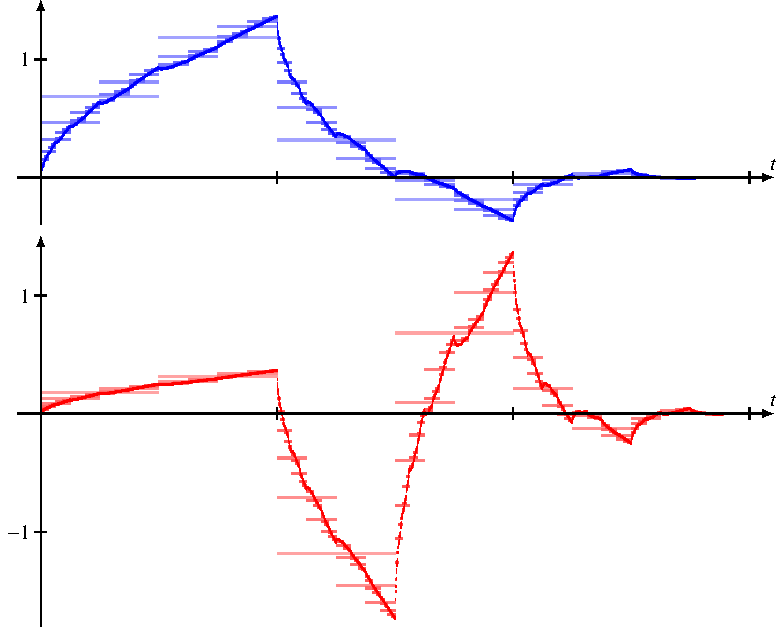
\includegraphics{chapters/7-algo/images/approx.pdf}
\caption{Approximation der Funktionen $\varphi$ (oben, blau) und
$\psi$ (unten, rot) für verschiedene
Werte von $j$ zwischen $1$ und $9$, dargestellt als Stufenfunktionen
mit zunehmen dunklerer Farbe.
\label{buch:algo:approx}}
\end{figure}
\begin{figure}
\centering
\begin{tikzpicture}
\node at (-2,0.50) {
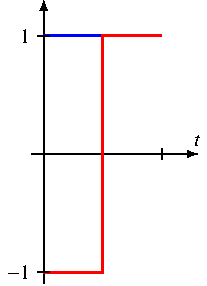
\includegraphics{chapters/7-algo/images/db1.pdf}
};
\node at (5,0) {
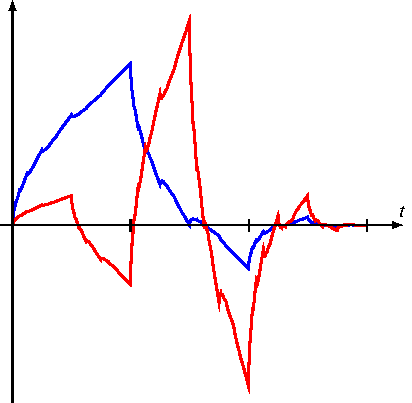
\includegraphics{chapters/7-algo/images/db2.pdf}
};
\end{tikzpicture}
\caption{Vater-Wavelet $\varphi$ (blau) und Mutter-Wavelet $\psi$
(rot) für die Daubechies-Wavelets \texttt{db1} und \texttt{db2}.
Das Daubechies-Wavelet \texttt{db1} ist identisch mit dem Haar-Wavelet.
\label{buch:algo:db1}}
\end{figure}%
\begin{figure}
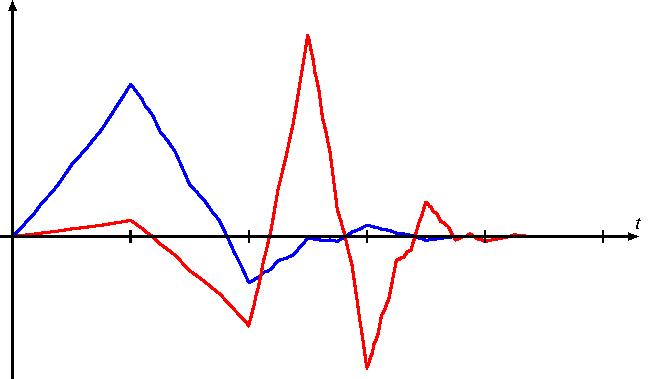
\includegraphics{chapters/7-algo/images/db3.pdf}\\
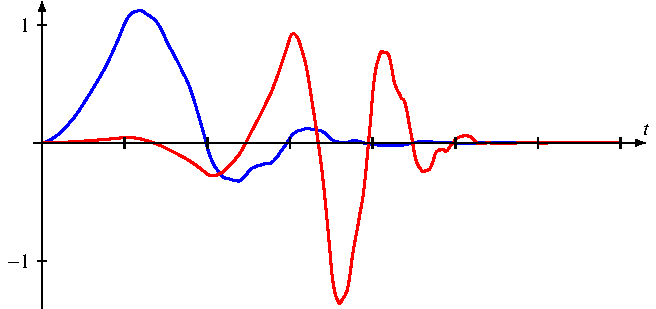
\includegraphics{chapters/7-algo/images/db4.pdf}\\
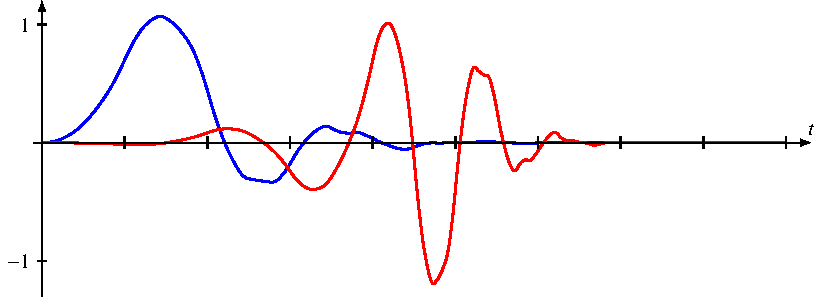
\includegraphics{chapters/7-algo/images/db5.pdf}
\caption{Vater-Wavelet $\varphi$ (blau) und Mutter-Wavelet $\psi$
(rot) für die Daubechies-Wavelets \texttt{db3} bis \texttt{db5}
von oben nach unten.
\label{buch:algo:db2}}
\end{figure}%
Für die praktische Anwendung einer Wavelet-Transformation ist
die konkrete Darstellung der Funktionen $\varphi$ und $\psi$
nicht notwendig.
Die schnellen Algorithmen sind völlig ausreichend um die
Koeffizienten $a_{j,k}$ und $b_{j,k}$ zu berechnen.
Ebenso kann die Umkehrtransformation mit belieger Genauigkeit
jedes Signal wieder rekonstruieren, ohne dass dazu explizit 
Linearkombinationen der Funktionen $\varphi$ und $\psi$ gebildet
werden müssten.

Trotzdem ist es interessant eine konkrete Vorstellung der Kurvenform
von $\varphi$ und $\psi$ zu haben, zum Beispiel um die in der
Wavelet-Transformation sichtbaren Features besser verstehen
zu können.
Dazu kann der schnelle Synthese-Algorithmus verwendet werden.
Ist nämlich $f(t)=\psi(t)$ das Mutter-Wavelet, dann gilt
\[
\begin{aligned}
a_{j,k}
&=
\langle \psi, \varphi_{j,k}\rangle = 0 
& &\text{für alle $j,k$}
\\
b_{j,k}
&=1&&\text{für $j=0$ und $k=0$}
\\
&=0&&\text{sonst.}
\end{aligned}
\]
Durch Anwendung der Rücktransformation können die Koeffizienten 
$a_{j,k}$ für beliebige Werte von $j$ und $k$ bestimmen.
Für genügend grosses $j$ sind die Koeffizienten $a_{j,k}$ im Wesentlichen
die Funktionswerte $\psi(k2^{-j}) = a_{j,k}$.
Auf analoge Weise können die Funktionswerte $\varphi(k2^{-j})$
rekonstruiert werden ausgehend von $a_{0,k}=\delta_{0k}$ für alle $k$
und $b_{j,k}=0$ für alle $j$ und $k$.
In Abbildung~\ref{buch:algo:approx} sind die verschiedenen Approximationen
für Werte von $j$ zwischen $1$ und $9$ dargestellt als Stufenfunktionen
mit zunehmend dunklerer Farbe.

Nach der Plancherel-Identität muss die Quadratsumme der Koeffizienten
$a_{j,k}$ eine gute Approximation für die Norm der analysierten Funktion
sein.
Je grösser $j$ ist, desto mehr Koeffizienten sind an der Quadratsumme
beteiligt und desto kleiner sind die einzelnen Koeffizienten.
Um die Funktionswerte zu rekonstruieren müssen die Koeffizienten
daher mit $2^{j/2}$ multipliziert werden.
Dies kann auch erreicht werden, indem man den schnellen Algorithmus
mit den Koeffizienten $\sqrt{2} h_k$ und
$\sqrt{2} g_k$ statt mit $h_k$ und $g_k$ durchführt.

In den Abbildungen \ref{buch:algo:db1} und \ref{buch:algo:db2}
ist das Resultat der Rücktransformation für die Daubechies-Wavelets
\texttt{db1} bis \texttt{db5} dargestellt.
Die Koeffizienten für die Skalierungsfunktionen dieser Wavelets werden
im Kapitel~\ref{chapter:kompakt} berechnet.

